\documentclass[tikz,border=10pt]{standalone}
\usepackage{tikz}
\usetikzlibrary{shapes.geometric, arrows}

\tikzstyle{startstop} = [rectangle, rounded corners, minimum width=3cm, minimum height=1cm,text centered, draw=black, fill=red!30]
\tikzstyle{process} = [rectangle, minimum width=3cm, minimum height=1cm, text centered, draw=black, fill=blue!30]
\tikzstyle{decision} = [diamond, minimum width=3cm, minimum height=1cm, text centered, draw=black, fill=green!30]
\tikzstyle{arrow} = [thick,->,>=stealth]

\begin{document}
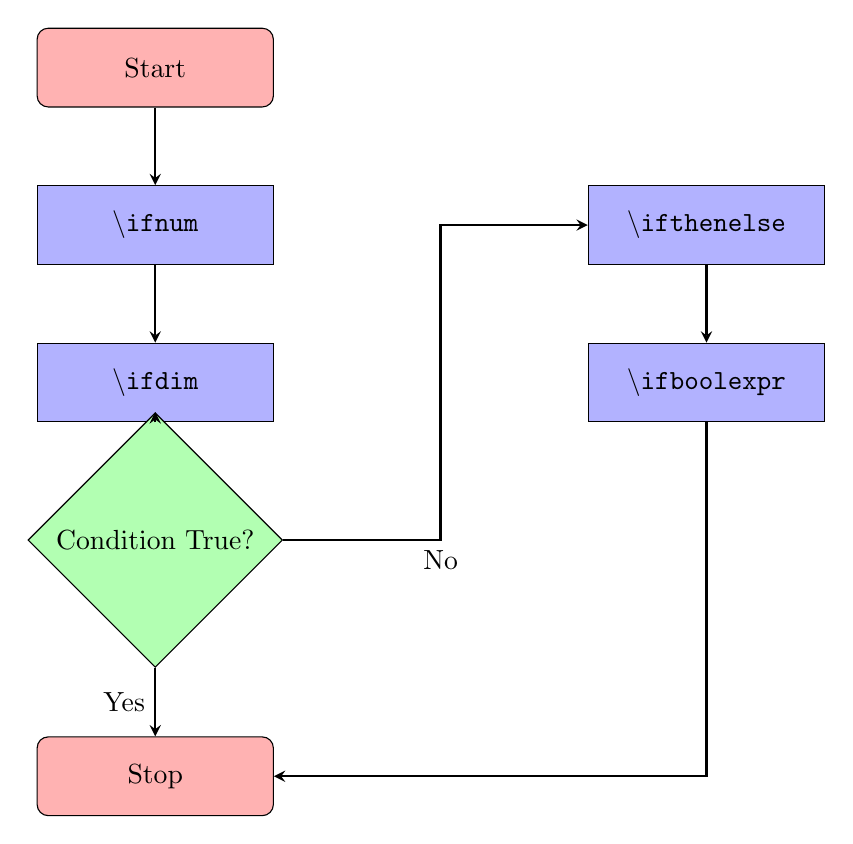
\begin{tikzpicture}[node distance=2cm]

% Nodes
\node (start) [startstop] {Start};
\node (ifnum) [process, below of=start] {\texttt{\textbackslash ifnum}};
\node (ifdim) [process, below of=ifnum] {\texttt{\textbackslash ifdim}};
\node (ifthen) [process, right of=ifnum, xshift=5cm] {\texttt{\textbackslash ifthenelse}};
\node (etoolbox) [process, below of=ifthen] {\texttt{\textbackslash ifboolexpr}};
\node (decision) [decision, below of=ifdim] {Condition True?};
\node (stop) [startstop, below of=decision, yshift=-1cm] {Stop};

% Arrows
\draw [arrow] (start) -- (ifnum);
\draw [arrow] (ifnum) -- (ifdim);
\draw [arrow] (ifdim) -- (decision);
\draw [arrow] (decision) -- node[anchor=east] {Yes} (stop);
\draw [arrow] (decision.east) -- ++(2,0) node[anchor=north] {No} |- (ifthen.west);
\draw [arrow] (ifthen) -- (etoolbox);
\draw [arrow] (etoolbox) |- (stop);

\end{tikzpicture}
\end{document}